\section{模型构建与实现}

\subsection{职业选择作为建模决策}

问题的前提要求从STEM、技工和艺术领域各选择一个职业。
我们没有将这一步骤视为临时假设（主观选择），而是明确地将职业选择建模为一个优化问题。
这确保了后续关于AI驱动影响和教育建议的分析建立在可重现且数据驱动的框架之上。
职业选择的核心目标不是所有职业的代表性，而是\emph{解释性对比}。
具体而言，三个职业的任务结构应当在与GenAI的交互方式上存在显著差异。
除了机制对比外，问题还明确强调数据驱动的推理以及后文的政策建议。因此，所选职业同时需要有完备的数据支撑以及政策相关性。

\subsubsection{基于O*NET的职业特征参数客观化}

为避免职业特征参数 $\textit{digit}(x)$、$\textit{physical}(x)$ 和 $\textit{iprisk}(x)$ 的主观赋值，我们采用美国劳工部维护的\textbf{O*NET}职业数据库作为统一数据源，详细的数据来源信息在第3节中总结。
O*NET基于专家调查和从业者反馈，为每个职业提供大量\emph{数值量表描述符}，大多数指标自然地给出在$0$--$100$之间的实数上，适合直接用于定量建模。

我们不试图为每个维度找到"唯一正确"的指标，对于每个特征轴，我们选择少量语义上直接对应且可下载的O*NET描述符，并将其用作该轴的代理变量。

基于问题陈述和数据可用性约束，我们识别出三个主导维度，这些维度控制着AI影响在各职业间的异质性：
\begin{itemize}
    \item \textbf{数字化程度$digit(x)$}：核心任务可以以数字方式表示、自动化或增强的程度；
    \item \textbf{物理锚定$physical(x)$}：任务执行对现场物理存在或与环境的手动交互的依赖程度；
    \item \textbf{知识产权和署名风险$iprisk(x)$}：价值创造对作者身份、原创性和所有权的敏感程度。
\end{itemize}

每个候选职业$x$由一个归一化的三维特征向量表示
\begin{equation}
    f(x)=\big(digit(x),\,physical(x),\,iprisk(x)\big)\in[0,1]^3,
\end{equation}
其中较高的值表示相应特征的存在更强。

对于分别从STEM、技工和艺术类别中抽取的三个职业类别 $(x_1,x_2,x_3)$，我们将两个职业之间的对比定义为其特征向量之间的欧几里得距离：
\begin{equation}
    \Delta(x_i,x_j)=\lVert f(x_i)-f(x_j)\rVert_2.
\end{equation}

定义数据可得性得分$D(x_k)$，反映获取该职业相关数据的难易度与丰富度。整体选择目标公式化为
\begin{equation}
    \max_{x_1\in STEM,\;x_2\in Trade,\;x_3\in Arts}
    \left(
    \sum_{i<j}\Delta(x_i,x_j)
    +\lambda\sum_{k=1}^{3}D(x_k)
    \right),
\end{equation}
其中 $\lambda$ 为权重系数，平衡解释性对比与经验可行性。

该公式不声称在所有可能职业中具有全局最优性。
相反，它产生一个精心构建的高对比度职业集，在现实数据和时间约束下最大化分析清晰度。

\paragraph{归一化与可重现性}
对于每个职业 $x$，令 $v_m(x)$ 表示其在O*NET描述符 $m$ 下的原始评分（$0$--$100$）。
我们在整个职业集上应用最小-最大归一化：
\begin{equation}
    z_m(x)=\frac{v_m(x)-\min_{y}v_m(y)}{\max_{y}v_m(y)-\min_{y}v_m(y)} \in [0,1],
\end{equation}
并对同一特征轴下的多个描述符取等权平均，得到 $\textit{digit}(x)$、$\textit{physical}(x)$ 和 $\textit{iprisk}(x)$。
该过程完全基于公开可用数据和明确规则，确保参数值的可重现性和可审计性。

我们可视化了三维异质性及其二维投影，以验证所选职业在特征空间中占据不同区域（图~\ref{fig:heterogeneity3d} 和图~\ref{fig:heterogeneity2d}）。

\begin{figure}[H]
\centering
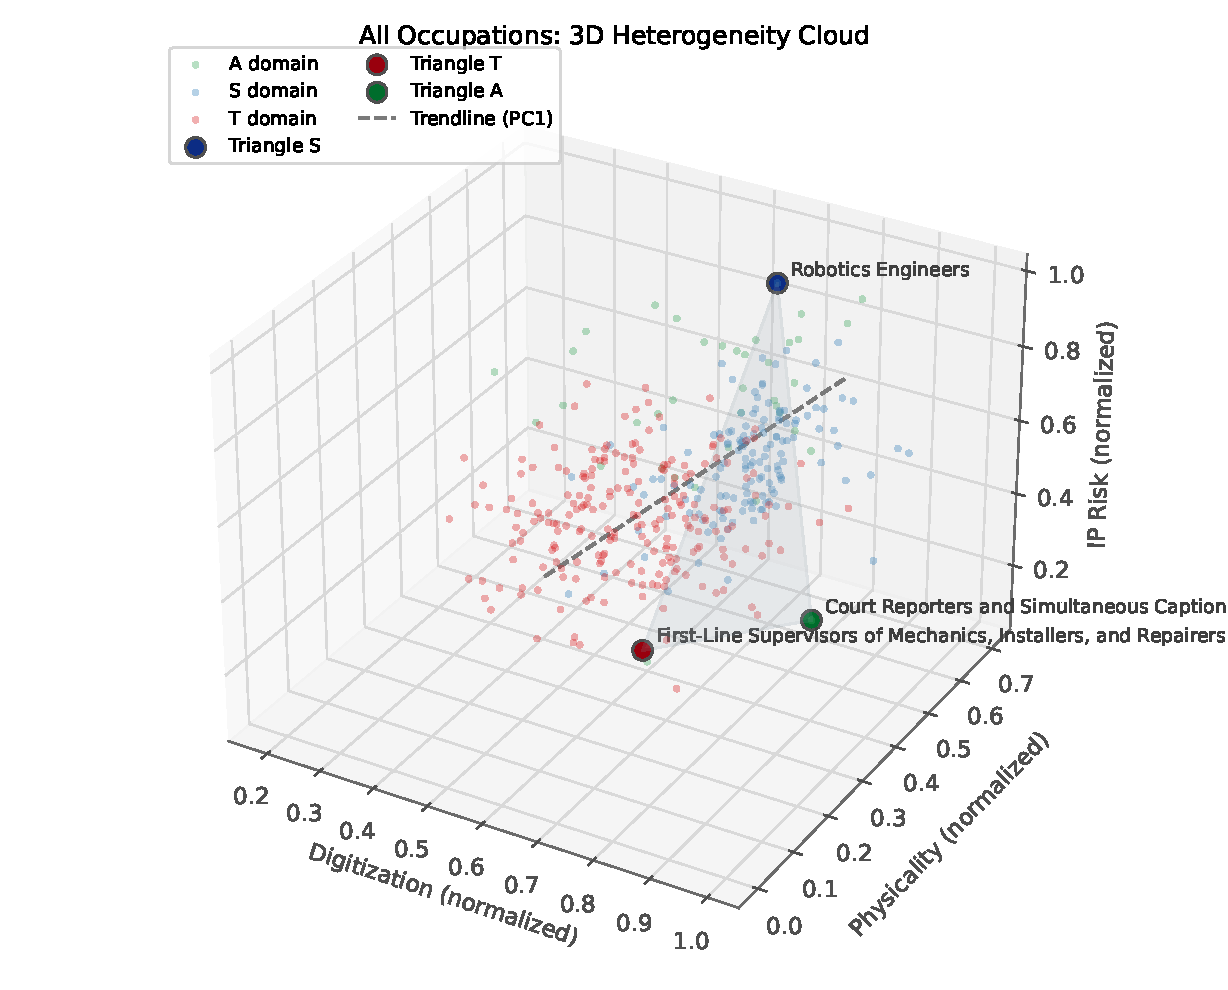
\includegraphics[width=0.78\textwidth]{figures/fig_heterogeneity_3d_all_points_strict.pdf}
\caption{基于O*NET描述符（全局归一化）的全体职业三维异质性点云与最优三角面（strict映射）。}
\label{fig:heterogeneity3d}
\end{figure}

我们先在全点云上求解无约束的最大面积三角形，随后根据赛题要求加入“STEM/技工/艺术三域各取一职”的约束，在可行域内重新最优化，得到约束后的最优三点：STEM（Robotics Engineers）、技工/Trades（First-Line Supervisors of Mechanics, Installers, and Repairers）与艺术/媒体（Court Reporters and Simultaneous Captioners）。其三角形面积为 $0.262221$，最短边长为 $0.751378$，该约束最优结果刻画三域职业在三维特征空间上的最大异质性跨度。

\vspace{0.6\baselineskip}

\begin{figure}[H]
\centering
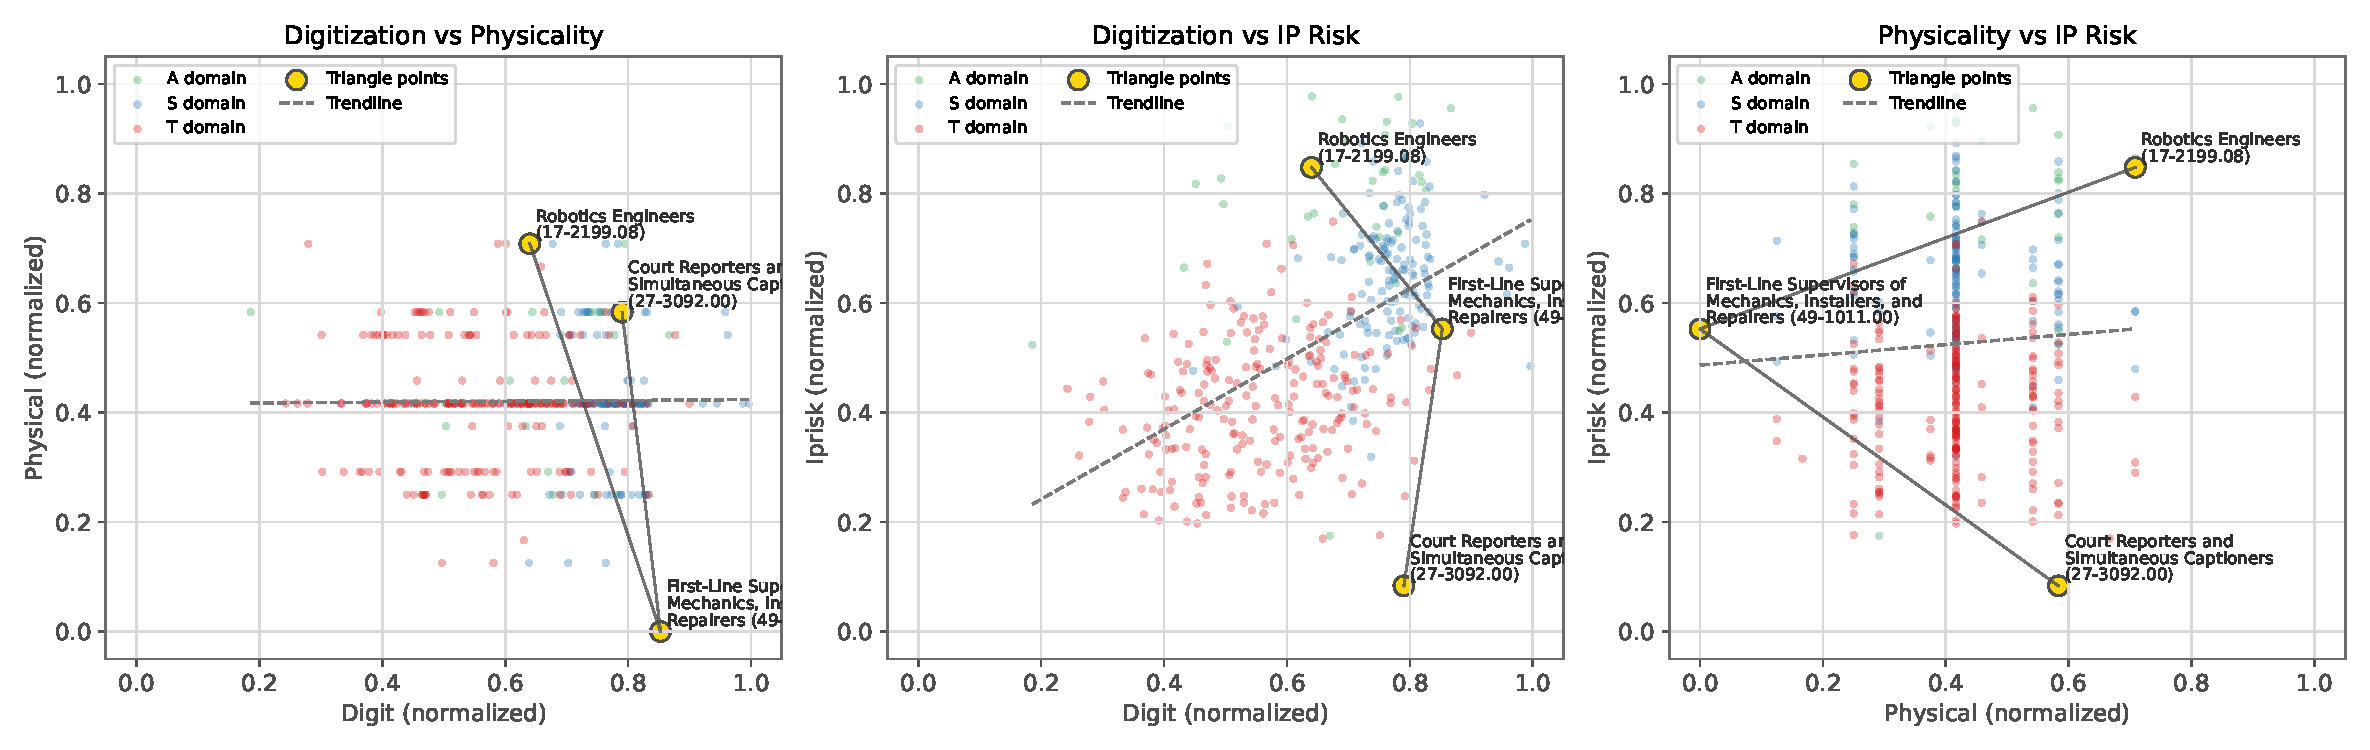
\includegraphics[width=0.92\textwidth]{figures/fig_heterogeneity_2d_projections_all_points_strict.pdf}
\caption{全体职业异质性空间的二维投影与最优三点标注（strict映射，全局归一化）。}
\label{fig:heterogeneity2d}
\end{figure}

\subsubsection{所选职业的修订与最终配置}

在初始方案中，我们选择结构/土木工程师作为STEM职业。然而，在进一步检查三个职业在"任务结构"和"物理约束"维度上的分布后，我们发现该选择与技工职业（电工）在"物理锚定强度"轴上存在一定相似性，可能削弱三个职业在机制空间中的对比度。

为最大化任务结构异质性并增强后续GenAI影响机制的可识别性，我们修订STEM端点，将其替换为\textbf{软件开发人员/软件工程师}。

该修订不改变原始选择模型的结构，仅调整职业端点在特征空间中的位置：软件开发人员具有极高的数字化程度和极低的物理锚定，从而显著增加其与电工在特征向量 $f(x)$ 中的距离，提高整体对比目标函数的值。

必须强调的是，我们不假设软件开发职业会被GenAI简单"替代"。相反，该职业更可能经历\textbf{任务结构重组}：编码和样板实现的比例降低，而需求澄清、系统架构设计、验证测试以及安全合规职责等任务的比例增加。正是这种从"执行导向型任务"到"验证和责任导向型任务"的转变，使软件开发成为研究GenAI影响机制的理想STEM端点。

完成此修订后，三个所选职业的最终配置如下：

\begin{itemize}
    \item \textbf{STEM：软件开发人员/软件工程师。}  
    数字化程度高，物理锚定低；GenAI可直接介入核心任务，但主要表现为任务再分配而非职业消亡。

    \item \textbf{技工：电工。}  
    物理锚定高，现场约束强；AI主要作为规划、诊断和辅助工具，难以替代核心操作任务。

    \item \textbf{艺术：商业插画师/平面设计师。}  
    知识产权和署名敏感性高；GenAI直接影响产出形式和价值定价机制。
\end{itemize}

\subsection{职业演化的模型选择}

问题的第二个核心要求是构建一个\emph{数据驱动}的未来职业演化模型。
在引入正式方程之前，我们首先定义"未来演化"在可计算意义上的含义，然后系统地评估替代建模方法，使模型选择本身不成为隐式假设。

\subsubsection{未来演化的可计算定义}

我们将职业 $i$ 的未来演化刻画为两个主要输出：
\begin{itemize}
    \item \textbf{职业需求}：在快速、中速和慢速GenAI采纳情景下，就业需求 $E_i(t)$ 在10年期限内的时间演化；
    \item \textbf{任务结构}：职业内任务权重 $T_i(t)$ 的重新分配，表明哪些任务扩展、收缩或被重组。
\end{itemize}

该定义确保职业级结果源自任务级机制，而非直接施加。

\subsubsection{候选建模方法比较}

我们考虑三种代表性的职业演化建模方法：

\paragraph{方法A：任务聚合影响模型}
该方法将职业视为任务的加权组合。
GenAI驱动的替代和增强效应在任务级指定，然后使用任务权重聚合到职业级。
大多数参数可从O*NET任务数据 \cite{onet2025database} 和公开可用的AI暴露标尺 \cite{freyosborne2017} 构建，提供透明性和可重现性。

\paragraph{方法B：招聘信息时间序列模型}
该方法从招聘信息中AI相关关键词和技能要求的趋势推断职业变化。
虽然与市场信号紧密相关，但它存在识别挑战和高数据处理开销，不适合作为主要建模骨架。

\paragraph{方法C：基于代理的模拟}
基于代理的模型模拟企业、工人和教育机构之间的战略互动。
尽管叙事丰富，但它们需要大量校准并引入实质性模型复杂性，这与严格页数限制下的透明性要求相冲突。

\subsubsection{最终模型选择}

基于上述比较，我们采用任务聚合影响模型（方法A）作为主要框架。
该选择的动机是：
\begin{itemize}
    \item \textbf{机制清晰性}：职业变化明确源自任务级效应；
    \item \textbf{数据对齐}：关键参数基于公开可用的职业数据 \cite{onet2025database,censuspseo2025}；
    \item \textbf{复杂性可控}：模型保持可解释性，适合情景和敏感性分析；
    \item \textbf{可迁移性}：框架可容易地扩展到其他职业或教育路径 \cite{ncescip2020soc2018}。
\end{itemize}

方法B保留用于潜在验证或补充分析，而方法C由于校准和透明性问题被排除在主要分析之外。

\subsection{职业演化的任务聚合动态模型}

在论证了任务聚合方法之后，我们现在展示其数学公式。
我们采用一个最小化的任务到职业框架：GenAI采纳 $A(t)$ 作为外生驱动因素进入，替代和增强在任务级指定，职业级净影响通过任务权重聚合得出，产生职业需求 $E_i(t)$ 的动态轨迹。

\subsubsection{任务聚合与职业动力学}

设职业 $i$ 由任务 $j=1,\dots,J_i$ 组成，权重为 $w_{ij}$，满足
\begin{equation}
    \sum_{j=1}^{J_i} w_{ij} = 1.
\end{equation}
对于每个任务 $j$，令 $s_{ij}\in[0,1]$ 表示替代强度，$c_{ij}\in[0,1]$ 表示增强（互补性）强度。
定义职业级聚合效应为
\begin{equation}
    \alpha_i=\sum_{j=1}^{J_i} w_{ij}\,s_{ij},\qquad
    \beta_i=\sum_{j=1}^{J_i} w_{ij}\,c_{ij}.
\end{equation}

令 $E_i(t)$ 为职业 $i$ 在时刻 $t$ 的就业需求，$g_i$ 捕获非AI因素的基线增长/衰减（从公共趋势估计或在情景分析下设为 $0$）。
给定采纳轨迹情景族 $A(t)\in[0,1]$（快速/中速/慢速），我们将职业演化建模为
\begin{equation}
    \frac{dE_i(t)}{dt}=E_i(t)\Big(g_i + A(t)\,(\beta_i-\alpha_i)\Big).
\end{equation}
该公式确保职业结果源自任务级机制，支持可解释性、可重现性和数据驱动推理。

\subsection{来自权威报告的GenAI能力维度评分：量表定义与证据叙述}

为取代主观的"关键词标签"方法，我们采用来自权威评估和官方技术报告的能力评分。
这些评分量化了GenAI在主要软件开发任务维度上的\textbf{替代}和\textbf{增强}能力，为将软件开发人员任务DNA映射到 $(s,c)$ 输入提供可审计的依据。

\subsubsection{量表定义}

我们使用三个级别（低/中/高）表示GenAI能力，编码为 $0.25$、$0.50$ 和 $0.75$：
\begin{itemize}
    \item \textbf{低（0.25）}：GenAI在该任务类型上的自主能力有限，无法在没有人工干预的情况下可靠地交付满意结果；只能替代一小部分工作，但在人工监督下仍可提供协助。
    \item \textbf{中（0.50）}：GenAI表现中等，完成部分任务或提供有用建议，但仍需人工审查和协作；无法独立替代人工执行。
    \item \textbf{高（0.75）}：GenAI表现强劲，在许多子任务上接近专业人类水平；在适当约束和验证下，可处理大部分工作流程并提供显著增强，但仍不完美。
\end{itemize}

\noindent\textbf{注意：}$0.25/0.50/0.75$ 的值是粗略的建模编码而非精确测量。所有级别都基于过去两年内发布的公开报告和对比实验。

\subsubsection{按任务类型的能力证据（叙述性论证）}

\paragraph{代码生成}
\textbf{替代：高（0.75）；增强：高（0.75）。}
GenAI在自动代码生成方面取得了强劲表现。OpenAI GPT-4在HumanEval上达到 $67.0\%$ pass@1，远高于GPT-3.5的 $48.1\%$；Anthropic Claude 2在同一基准上达到 $71.2\%$。这表明领先模型能正确解决超过一半的典型编码问题。Google CEO Sundar Pichai表示，Google约 $25\%$ 的新代码由AI工具生成，反映出显著的生产力提升：给定意图或注释，模型可以生成大量草稿代码并加速开发。对于简单模块，模型可以部分替代手动编码。然而，输出仍需人工审查和测试以减少逻辑错误和安全问题。总体而言，编码/实现是GenAI最具替代性和增强性的领域之一。

\paragraph{测试与验证}
\textbf{替代：中（0.50）；增强：高（0.75）。}
GenAI在生成测试用例和支持验证方面表现中等但在改进。研究报告显示，LLM生成的单元测试可以达到与先进自动化工具相当的覆盖率，且通常更具可读性。例如，IBM研究院在静态分析引导下的实验发现，基于GPT的系统可以生成具有竞争力覆盖率和缺陷检测能力的Java/Python单元测试，同时产生对开发者友好的测试。这支持了在常规函数级验证中的强劲增强。然而，生成的测试可能针对不相关场景或弱断言，需要人工审查；因此完全替代仍然困难。在实践中，GenAI可以大幅减少手动测试编写并加速结果检查，而人类验证测试正确性。

\paragraph{调试与错误修复}
\textbf{替代：低（0.25）；增强：中（0.50）。}
端到端调试仍是弱项：自主成功率相对较低，但辅助价值明显。2025年Microsoft Research的一项研究报告显示，即使有调试器工具访问，最佳模型（Anthropic Claude 3.7 Sonnet）平均只解决了300个精选调试任务中的 $48.4\%$，而其他模型约为 $30\%$。这表明GenAI无法完全替代人工调试。局限性包括对调试信号的无效使用、策略选择不当以及缺乏逐步推理痕迹。因此替代被评为低。同时，增强是明显的：有了日志或异常跟踪，模型可以提出有用的修复建议；在某些设置中，通过少样本演示的"自我调试"可提高约 $2\%$--$12\%$ 的成功率。在实践中，GenAI更多地作为助手而非独立的"修理工"。

\paragraph{系统设计/架构}
\textbf{替代：低（0.25）；增强：中（0.50）。}
架构和系统设计需要全局推理和负责任的权衡；GenAI目前提供有限的支持。虽然没有单一的权威基准直接衡量系统设计能力，但模型通常产生看似合理但不完整的计划，遗漏关键约束或依赖错误假设。由于系统设计没有单一正确答案且需要负责任的决策，自主替代被评为低。尽管如此，增强可能有意义：模型可以起草设计文档、总结模式并头脑风暴替代方案，作为架构师的起点，提高讨论效率。

\paragraph{需求分析}
\textbf{替代：低（0.25）；增强：中（0.50）。}
需求工作需要深入的领域背景和歧义消解。GenAI可以协助总结和结构化文本，但无法替代分析师。虽然专门评估有限，但相关任务如自然语言到形式化规范提供了证据：在Spider（自然语言到SQL）上，即使使用增强技术，GPT-4的提升仅约 $2\%$--$3\%$，复杂查询仍具挑战性。这意味着对复杂、模糊需求的理解不可靠，因此替代为低。然而，增强是中等的：模型可以总结冗长文档、生成用户故事模板、提出澄清问题，并在人工监督下加速需求组织。

\paragraph{用户沟通与文档}
\textbf{替代：中（0.50）；增强：高（0.75）。}
GenAI在语言生成方面表现出色，强力增强用户沟通和技术文档。GPT-4和Claude 2等模型可以生成连贯的长篇草稿并遵守结构化格式（如Markdown/JSON），实现API文档、手册和用户响应的快速起草。许多常规用户查询可以流畅且一致地回答。然而，准确性和幻觉风险仍然存在，特别是对于系统特定细节，因此完全替代人工沟通仍有风险；替代被评为中而增强被评为高。

\begin{table}[htbp]
\centering
\caption{来自权威评估报告的GenAI能力维度标尺（用于将软件开发人员任务映射到 $s/c$）}
\label{tab:genai_capability_rubric_en}
\begin{tabular}{p{2.6cm} p{2.2cm} p{2.2cm} p{7.2cm}}
\toprule
任务类型 & 替代得分 & 增强得分 & 主要证据和支持 \\
\midrule
\textbf{代码生成} & 高（0.75） & 高（0.75） &
GPT-4在HumanEval上达到67.0\% pass@1 \cite{openai2023gpt4}。\newline
Claude 2达到71.2\% \cite{anthropic2023claude2}。\newline
Google报告约25\%的新代码由AI生成 \cite{techcrunch2025aimodels}。 \\
\textbf{测试与验证} & 中（0.50） & 高（0.75） &
LLM生成的单元测试可达到有竞争力的覆盖率和可读性。\newline
研究表明在静态分析引导下测试质量更高 \cite{arxiv2024unittest}。\newline
仍需人工审查，因此替代保持中等。 \\
\textbf{调试与错误修复} & 低（0.25） & 中（0.50） &
Microsoft Research报告即使有调试工具，端到端调试成功率低于50\%（最佳模型48.4\%）\cite{techcrunch2025aimodels}。\newline
提示修复建议有帮助，"自我调试"可提高准确率最多12个百分点 \cite{chen2023selfdebugging}。 \\
\textbf{系统设计} & 低（0.25） & 中（0.50） &
复杂架构需要综合推理；当前GenAI通常产生部分解决方案 \cite{openai2023gpt4}。\newline
直接定量基准有限，但模型可以协助起草和文档以加速设计讨论 \cite{googleresearch2024seqmodels}。 \\
\textbf{需求分析} & 低（0.25） & 中（0.50） &
模型在NL$\rightarrow$spec任务上的提升有限（如Spider上2--3\%）\cite{chen2023selfdebugging}。\newline
然而，总结和问题生成可以提高需求获取和分析效率 \cite{openai2023gpt4}。 \\
\textbf{用户沟通与文档} & 中（0.50） & 高（0.75） &
Claude 2等模型可以高效生成长篇结构化文档并回答常见问题 \cite{anthropic2023claude2}。\newline
准确性仍是问题；关键内容仍需人工验证 \cite{openai2023gpt4}。 \\
\bottomrule
\end{tabular}
\end{table}

\subsection{任务影响的权威评估驱动重标记：从关键词标签到能力维度分配}

为提高任务影响参数 $(s_{ij},c_{ij})$ 的可辩护性和可重现性，我们放弃主观关键词标签，
采用"\textbf{权威评估 $\rightarrow$ 能力维度 $\rightarrow$ 语义匹配 $\rightarrow$ 分段分配}"的重标记工作流。
核心思想是从官方评估报告中提取一组\emph{能力维度}（如代码生成、调试、测试/验证、需求分析、系统设计、文档/沟通）的替代/增强级别，
将每个软件开发人员任务映射到1--2个能力维度，然后在离散网格上分配 $(s_j,c_j)$。

\paragraph{能力映射与可追溯性要求}
对于每个任务 $j$，定义其映射的能力集 $\textit{dim}_j$（通常为1--2个维度以保持可解释性）。
任务级替代和增强在离散量表上分配：
\begin{equation}
s_j,\ c_j\in\{0.25,\ 0.5,\ 0.75\}.
\end{equation}
为满足"数据驱动"审计标准，每个任务必须携带\textbf{可追溯链}：(i) 映射的能力维度 $\textit{dim}_j$，(ii) 至少一个权威来源链接，(iii) 任务到维度匹配逻辑的简要说明。
这确保 $(s_j,c_j)$ 是可审查的而非基于研究者直觉。

\paragraph{语义阈值、异常报告与有限人工覆盖}
由于语义匹配可能导致漏报和误报，匹配阈值被视为可控决策参数：
阈值过高可能遗漏有效匹配；过低可能引入错误匹配。
因此，重标记输出必须包含相似度得分和异常报告（如低相似度匹配、多维度分配冲突），并允许对少量语义模糊的高权重任务进行小规模人工覆盖列表。
这保持了整体可重现性，同时防止少量错误标签偏移职业级聚合值 $(\alpha_i,\beta_i)$。

\subsection{将任务DNA聚合为职业级冲击参数：软件开发人员}

本节将软件开发人员任务DNA从任务级输入 $(w_{ij}, s_{ij}, c_{ij})$ 聚合为职业级冲击参数 $(\alpha_i,\beta_i,\mu_i)$，
这将输入演化方程 $\frac{dE_i(t)}{dt}=E_i(t)\big(g_i + A(t)(\beta_i-\alpha_i)\big)$。

\subsubsection{Top-$N$ 可用性与聚合}

在实践中，O*NET任务评分可能对某些任务缺失。
因此我们采用"Top-$N_i$ 可用任务"策略：对于职业 $i$，我们只保留具有足够评分以构建权重的任务，并重新归一化使得 $\sum_{j=1}^{N_i} w_{ij}=1$。
职业级替代压力、增强收益和净方向定义为
\begin{equation}
    \alpha_i=\sum_{j=1}^{N_i} w_{ij} s_{ij},\qquad
    \beta_i=\sum_{j=1}^{N_i} w_{ij} c_{ij},\qquad
    \mu_i=\beta_i-\alpha_i.
\end{equation}

\subsubsection{可解释性分解：Top-$K$ 贡献下界}

为增强可解释性，我们分解高权重任务的贡献。定义部分和
\begin{equation}
    \alpha_i^{(K)}=\sum_{j\in \text{Top-}K} w_{ij}s_{ij},\qquad
    \beta_i^{(K)}=\sum_{j\in \text{Top-}K} w_{ij}c_{ij}.
\end{equation}
对于当前可用的Top-5样本，$\sum_{j\in \text{Top-}5} w_{ij}=0.360897$，
部分贡献 $\alpha_i^{(5)}=0.1804485$ 和 $\beta_i^{(5)}=0.2153186$，
表明高权重任务（通常是测试/维护/需求/协作）将主导聚合冲击。

\subsubsection{评分规则的有效性检验：避免近常数 $s/c$}

如果许多任务共享相同的离散得分（如 $0.50$），则 $\alpha_i$ 和 $\beta_i$ 变得弱区分性，削弱机制解释。
因此我们检验离散网格 $\mathcal{G}=\{0,0.25,0.5,0.75,1\}$ 上的权重质量集中度：
\begin{equation}
    p_s(g)=\sum_{j:\,s_{ij}=g} w_{ij},\qquad
    p_c(g)=\sum_{j:\,c_{ij}=g} w_{ij},\qquad g\in\mathcal{G},
\end{equation}
使用集中度和归一化熵：
\begin{equation}
    C_s=\max_{g\in\mathcal{G}} p_s(g),\qquad
    C_c=\max_{g\in\mathcal{G}} p_c(g),
\end{equation}
\begin{equation}
    H_s=-\frac{\sum_{g\in\mathcal{G}} p_s(g)\ln p_s(g)}{\ln|\mathcal{G}|},\qquad
    H_c=-\frac{\sum_{g\in\mathcal{G}} p_c(g)\ln p_c(g)}{\ln|\mathcal{G}|}.
\end{equation}
高 $C_s$ 或低 $H_s$ 标志得分压缩并触发最小校准。

\subsubsection{最小校准：带有限人工审查的类别默认值}

为避免重新收集数据，我们仅通过一小组任务类别校准 $s/c$，同时保持任务列表和权重 $w_{ij}$ 不变。
令 $\kappa(j)$ 将每个任务映射到一个粗类别（如需求/利益相关者、编码/实现、测试/验证/安全、监控/运维），并带有默认 $(s,c)$ 对。
然后我们仅手动审查少量高权重任务并记录简要证据说明，在保持可重现性和透明性的同时提高 $(\alpha_i,\beta_i)$ 的可识别性。
